% \VignetteDepends{stats}
% \VignetteIndexEntry{Report on side effect risks in hospital}
% \VignetteKeywords{htest}
% \VignettePackage{rhosp}



\documentclass[12pt,twoside]{article}

\usepackage{epsfig}
\usepackage{latexsym}
\usepackage{amsxtra}
\usepackage{vmargin}
\usepackage{amsfonts,amsmath,amssymb,amsthm}
\usepackage{color,graphics}
\usepackage{courier}
\usepackage{newlfont}

\usepackage[noae]{Sweave}


%\usepackage[frenchb]{babel}
\usepackage[latin1]{inputenc}
\usepackage{graphicx}


%mise en page
\pagestyle{headings}
% \setlength{\marginparwidth}{0pt}




% les macros
\newcommand{\II}{\mbox{\large 1\hskip -0,353em 1}}
\newcommand{\abs}[1]{\lvert#1\rvert}
\newcommand{\norm}[1]{\lVert#1\rVert}
\newcommand{\ligne}{\rule[2mm]{.3\textwidth}{0,5mm}\\}
\renewcommand{\emph}{\textbf}
\newcommand{\sigle}{\textsc}
\newcommand{\email}{\texttt}
\newcommand{\software}{\textsc}
\newcommand{\myskip}{\vspace{\parskip}}

%-----------------------------------------------------------------------

\title{\vspace{-1.5cm}
{\normalsize Projet de sp\'ecialit\'e \hfill
       $2^{\grave{e}me}$ ann\'ee \sigle{ensimag}, 2005~--~2006}
       \\[5cm]
	\textsf{An actuary approach of risk evaluation during hospitalizations}}
\vspace{2.5cm}
\author{Julie Barthés \and Christophe Dutang}



%==========================================================
\begin{document}
%==========================================================

\setpapersize{A4}

\addtolength{\parskip}{2mm}
\maketitle
\date
\newpage
\tableofcontents 
\newpage

\section{Introduction}
\label{introduction}

Cost control is nowadays one of health services major concerns. They put a stake on hospitalization management. 
Indeed, they are interested in the conditions of patients stays, in order to create a new hospitalization policy. Moreover, physicians take an interest in the occupancy of hospital beds because its study could help to prevent patients from side effects such as venous thrombosis, nosocomial infections, etc. A risk process can be observed and quantified. This risk estimation is at stake in our work.\\

Such a study is to be seen in the context of modelling concrete issues that involve random events. 
We use an actuary approach in the collective risk theory in order to submit an evaluation of risk during hospitalizations. We also deliver an \texttt{R} package of risk estimation during hospitalization.\\

In section \ref{methods}, we model the stay of a patient in hospital defining the probability that a patient reports a side effect and the duration of an healthy stay. Moreover, we assume that the fact that a side effect arises depends on the duration of the stay. This is the \textsl{model with conditioned side effects}. Then, we put forward the hypothesis that a side effect arises at a random instant : this builds up the second model named \textsl{model with random side effects}. In both models, we get some explicit results in particular cases. Thus, using risk theory and renewal findings, we are able to express a \textsl{risk constant} $R$ that ensures the knowledge of a \textsl{survival function} of patients at infinity.\\

However, in most cases, we are not able to write an explicit expression of the risk constant $R$. That is why we subsequently study in section \ref{result} different methods in order to get an estimator of $R$ or the survival function and to quantify and value his quality. The De Vielder's approximation and the Kaplan-Meier's method are the most known ones. Then, we study the parameter inference of the risk constant using the likelihood function or the Bayes' formula. These methods seem to be suitable ones. \\

Finally, in section \ref{package}, we present an \texttt{R} package named \texttt{rhosp} dealing with risk during hospitalization. \texttt{rhosp} contains functions to evaluate and simulate the risk constant. 





\clearpage
%%%%%%%%%%%%%%%%%%%%%%%%%%%%%%
% MODEL 1
%%%%%%%%%%%%%%%%%%%%%%%%%%%%%%

\section{Methods and techniques to get the risk constant}
\label{methods}
In this section, we study two models and distributions in order to bring out theoretical results about risks during hospitalization.\\

Evaluating risk during hospitalization, it seems logical to include as a parameter the durations of the patient stays in the model. Indeed, each $X_i$ stands for the time spent in hospital. We suppose that $X_i$ is exponentially distributed with a parameter $\lambda$ so that 
$1/\lambda$ expresses the mean length of a patient hospitalization. Assuming that a patient stays at least one day in hospital, we will choose $\lambda$ in $(0,1)$.\\



Moreover, it seems reasonable to suggest that the fact that a side effect arises depends on the duration of the stay. Actually, the longer patients stay in hospital, the less combative against side effects they are. This is our first model : the model with conditioned side effects, clarified in figure \ref{mod1}. Nevertheless, we could put forward that reporting a side effect is simply bad luck. Thus, a side effect arises at a random instant. This is then our second model : the model with random side effects, clarified in figure \ref{mod2}. In both models, we need to give the probability that a patient reports a side effect given the duration of the treatment. That is why we introduce an element $p$ that expresses this probability and that is named \textsl{side effect probability}.


\subsection{Model with conditioned side effects}
We focus on the duration of a patient stay in hospital.  We look at one hospital bed and we observe 
the successive times of stay. These data are independently and identically distributed variables, which make 
up a renewal process. In the model with conditioned side effects, we assume the fact that a side effect arises depends on the duration of the stay.\\

The figure \ref{mod1} represents the model with conditioned side effects.\\


In this first model, we consider : 
\begin{itemize}
	\item a sequence of $(X_i)_i$ of independant and identically distributed random variables, having the 
		common distribution function $F$, with $F(0)=0$.
		The $(X_i)_i$ variables stand for the successive durations of the treatment for a patient and make up a renewal process.
	\item a sequence of $(Z_i)_i$ of independant and identically distributed random variables, having the 
		Bernoulli distribution with success probability $p(x)$. $p$ is a probability and is worth $1-q$, id est $p(x)=1-q(x)$.
		$p(x)$ is named side effect probability. It is the probability that a patient reports a side effect given that the treatment lasts $x$.	
	\item the random variable $N$ associated with the number of patients between two full-blown side effects.
\end{itemize}

The time of the first event, id est the first time when $Z_i$ is worth 1, is defined by:
$$T=\sum_{i=1}^{N}{X_i}$$ 
Its distribution function is $F_T(t)$ over the interval $(0,+\infty)$. For convenience, we use:
$$A(t)=P(T>t)=1-F_T(t)$$

$A(t)$ is the \textsl{survival function}. Its limit when the time is infinite is studied. The risk constants $R$ and $C_R$ 
are defined so that $A(t)$ has an exponential tail written $C_R e^{-R t}$ and named the \textsl{tail survival function}.
 

Several studied cases follow.


\begin{figure}[htb!]
\begin{center}
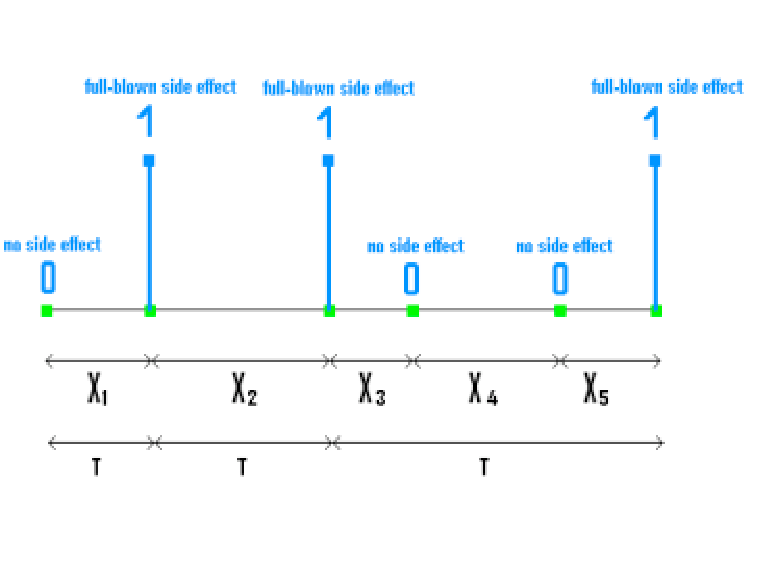
\includegraphics[width=12cm]{mod1.pdf} 

\caption{ The $(X_i)_i$ are the successive durations of treatment for five patients on the same hospital bed. At the end of each treatment, the $(Z_i)_i$ are worth $0$ or $1$ : the patient does not report any side effect or he has a full-blown one. }
\label{mod1}
\end{center}
\end{figure}


\subsubsection{A constant side effect probability}
We study a sequence of $(X_i)_i$ that has an exponential distribution with parameter $\lambda$ and a sequence of $(Z_i)_i$ that has a Bernoulli distribution with a constant side effect probability $p$. We focus on the model with conditioned side effects and with a constant side effect probability.\\

In this case, we can conclude that $T$ has an exponential distribution with 
parameter $\lambda p$ (as shown in appendix \ref{mod1_dem1} page \pageref{mod1_dem1}), thanks to the Laplace transform of a random variable. Thus, the survival 
function is worth $A(t)=e^{-\lambda p t}$. Moreover, $N$ has a geometric distribution with parameter $p$.\\

We have a theoretical expression of the risk constants $R$ and $C_R$ :
\begin{equation}
R=\lambda p ~\textrm{  and  } ~ C_R=1
\label{eq_mod1_exp_cst}
\end{equation}


See the figure \ref{cst} in section 3 for the simulation of this model.


\subsubsection{An exponential side effect probability}
We study a sequence of $(X_i)_i$ that has an exponential distribution with parameter $\lambda$ and a sequence of $(Z_i)_i$ that has a Bernoulli distribution with a side effect probability $p(x)=1-e^{-\mu x}$ having $\mu < \lambda$. We take an interest in the studyof the model with conditioned side effects and with an exponential side effect probability.

As shown in appendix \ref{mod1_dem2} page \pageref{mod1_dem2}, we are still able to express the survival function:
\begin{equation}
A(t)=\frac{1}{\lambda - \mu}(\lambda e^{-\mu t}-\mu e^{-\lambda t})
\label{eq_mod1_exp_exp_1}
\end{equation}
The mean and the second-order moment can be inferred from this equality.
$$E[T]=\frac{\lambda + \mu}{\lambda \mu}$$
$$E[T^2]=\frac{1}{\lambda^2}+\frac{1}{\lambda \mu}+\frac{1}{\mu^2}$$
That leads to a theoretical expression of the risk constants $R$ and $C_R$ :
\begin{equation}
R=\mu ~\textrm{  and  } ~C_R=\frac{\lambda}{\mu}(1-\frac{\lambda}{\mu-\lambda})
\label{eq_mod1_exp_exp_2}
\end{equation}


See the figure \ref{exp} in section 3 for the simulation of this model.

\subsubsection{An exponentially mixed side effect probability}
We study a sequence of $(X_i)_i$ that has an exponential distribution with parameter $\lambda$ and a sequence of $(Z_i)_i$ that has a Bernoulli distribution with a side effect probability $p(x)=1-p_1 e^{-\mu_1 x}-p_2 e^{-\mu_2 x}$. We focus on the model with conditioned side effects and with an exponentially mixed side effect probability.


We use the Laplace transform L and we look for $R$ so that $R$ is the smallest root of $(\star)$ : 
$$\lambda Lq(\lambda-R) = 1~~\quad(\star)$$  
Thus, we look for $R$  such as $$\sum_{i=1}^{2}\frac{p_i}{\mu_i+\lambda-R}=1$$
Then we have :
$$R=\frac{\mu_1+\mu_2+2\lambda-1 \pm \Delta}{2}$$
with $$\Delta=(\mu_1+\mu_2+2\lambda)^2-2(\mu_1+\mu_2+2\lambda)+1+4(p_1(\mu_2+\lambda)+p_2(\mu_1+\lambda)+(\mu_1+\lambda)(\mu_2+\lambda))$$


The resolution can also be done with $p(x)=1-\sum_{i=1}^{n}p_i e^{-m_i x}$ provided that we can solve a polynomial n-degree equation.

See the figure \ref{image_mod1_exp_comp} in section 3 for the simulation of this model.



\subsubsection{Any side effect probability}
We study a sequence of $(X_i)_i$ that has an exponential distribution with parameter $\lambda$ and a sequence of $(Z_i)$ that has a Bernoulli distribution with any side effect probability $p(x)$. We focus on the model with conditioned side effects and with any side effect probability.

We look for $R$ so that $R$ is the smallest root of: 
$$\lambda Lq(\lambda-R) = 1~~\quad(\star)$$

We suppose that $B(t)$ is such as :
$$B(t)=A(t)e^{Rt}$$

As shown in appendix \ref{mod1_dem3} page \pageref{mod1_dem3}, $B(t)$ verifies a renewal equation : \\
\begin{equation}
B(t)=b(t)+\int_0^t B(t-x)dG(x)
\label{renewal_eq}
\end{equation}
with $b(t)=e^{Rt}(1-F_T(t))$ and $dG(x) =g(x) dx =\lambda q(x) e^{-x(\lambda-R)}dx$

When $t\rightarrow +\infty$, $A(t)\sim C_R e^{-Rt}$
\begin{equation}
C_R=\frac{\lambda}{R}(1-\frac{\lambda}{R-\lambda})
\label{eq_mod1_exp_qcq}
\end{equation}

\subsubsection{General case}

We study a sequence of $(X_i)_i$ that has any density $f_{X_1}$ and a sequence of $(Z_i)$ that has a Bernoulli distribution with any side effect probability $p(x)$.

We can write the following equalities :
$$A(t)=1-F_{X_1}(t)+\int_{0}^{+\infty}A(t-x)q(x)f_{X_1}(x)dx$$

$$f_T(t)=f_{X_1}(t)-\frac{\partial}{\partial t}(\int_{0}^{+\infty}A(t-x)q(x)f_{X_1}(x)dx)$$

$$L_T(s)=L_{X_1}(s) - \int_{0}^{+\infty}(\frac{\partial}{\partial t}(\int_{0}^{+\infty}A(t-x)q(x)f_{X_1}(x)dx)e^{-st})dt$$


% transition : modèle 1 -> modèle 2
Here, in this subsection, the longer patients stay in a bed, the weaker they are in their fight against possible side effects. That was our model with conditioned side effects. Nevertheless, we could put forward that reporting a side effect is simply bad luck and happens at a random instant.


%%%%%%%%%%%%%%%%%%%%%%%%%%%%%%
% MODEL 2
%%%%%%%%%%%%%%%%%%%%%%%%%%%%%%
\subsection{Model with random side effects}
Like in the model with conditioned side effects, we focus on the duration of the stay of a patient in an hospital.


\subsubsection{Censored stay durations}  
We look at one hospital bed and we observe the successive times of stay. These data are independently 
and identically distributed variables, which make up a renewal process. In this model with random side effects, 
we assume  that a side effect arises at a random instant. This is depicted in figure \ref{mod2}.\\


In this section, we add a new sequence of random variables ($(Y_i)_i$) to the first model. Thus, we consider : 
\begin{itemize}
	\item a sequence of $(X_i)_i$ of independant and identically distributed random variables, 
		having the common distribution function $F_X$, with $F_X(0)=0$.
		The variables $(X_i)_i$ stand for the successive duration of the treatment for a patient and form a renewal process.
	\item a sequence of $(Y_i)_i$ of independant and identically distributed random variables, 
		having the common distribution function $F_Y$, with $F_Y(0)=0$.
		The variables $(Y_i)_i$ stand for the successive duration of exposure for a patient.
	\item a sequence of $(Z_i)_i$ of independant and identically distributed random variables, 
		having the Bernoulli distribution with success probability $p$:\\
		 $
Z_i =
\left\{
\begin{array} {lll}
1 & \textrm{if} & X_i > Y_i \\
0 & \textrm{if} & Y_i \geq X_i\\
\end{array}
\right.
$
		$p$ is the probability that the exposure duration $Y_i$ is shorter than the treatment exposure $X_i$ for the $i^{th}$ patient. 
	\item the random variable $N$ associated with the number of patients between two reported side effects.\\
\end{itemize}

\begin{figure}[htb!]
\begin{center}
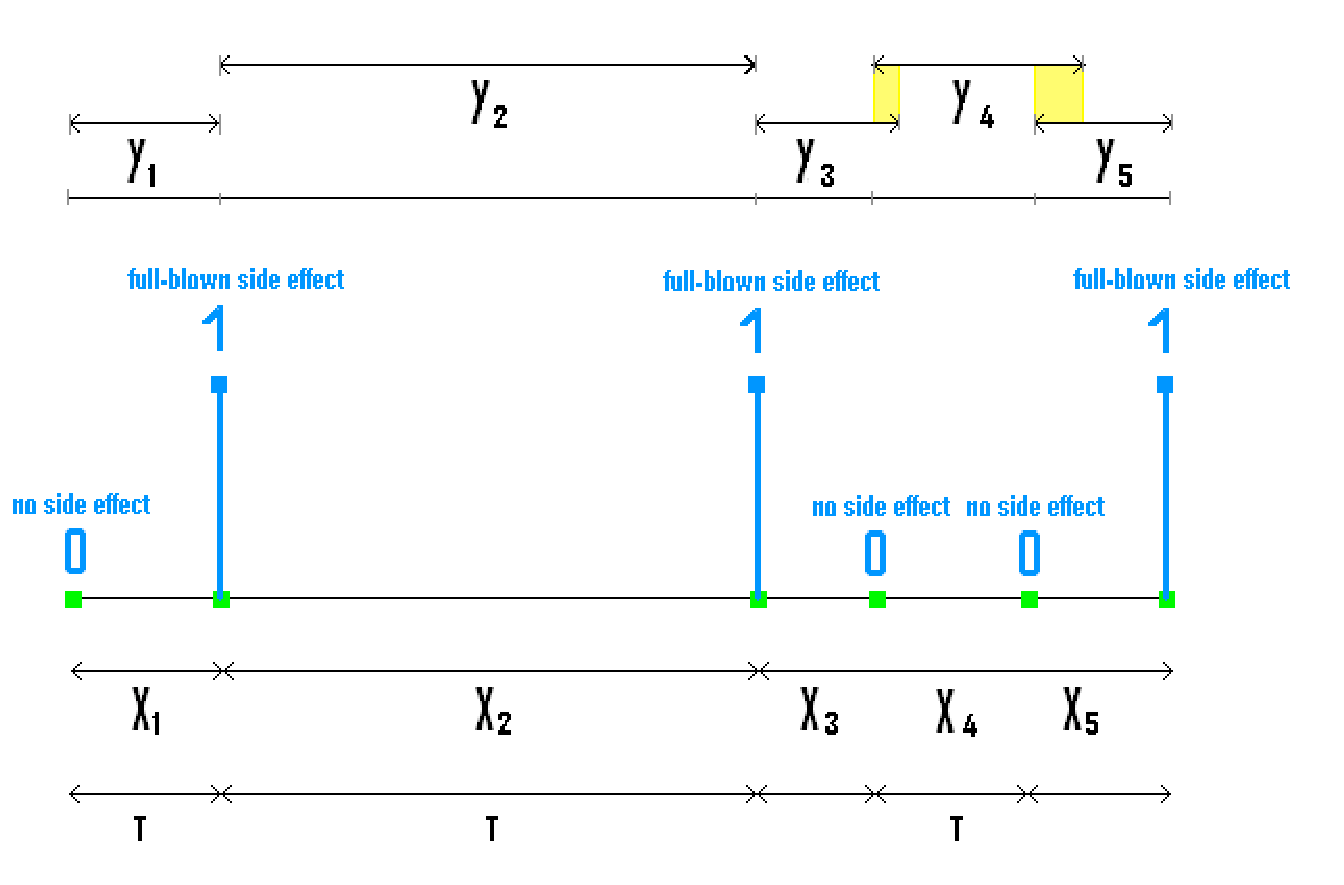
\includegraphics[width=14cm]{mod2.pdf} 

\caption{ The $(X_i)_i$ are the successive durations of treatment for seven patients on the same hospital bed. The $(Y_i)_i$ are the exposure duration. At the end of each treatment, the $(Z_i)_i$ are worth $0$ or $1$ : the patient does not report any side effect if $Y_i > X_i$ or he has a full-blown one if $Y_i < X_i$ (and then $X_i = Y_i$). }
\label{mod2}
\end{center}
\end{figure}



In our modelling, we choose to consider that a patient moves from his bed as soon as he has a full-blown side effect. That is to say that, if $Y_i < X_i$ then $X_i:=Y_i$ because $X_i$ is censored and $Z_i=1$. Had we considered that, if $Y_i < X_i$ then $X_i$ does not change, it would have lead us to the study of study of the model with conditioned side effects, with $p(x) =F_{Y_i}(x)$.




\subsubsection{Uncensored stay durations}
As explained above, if we suppose that the sequence of $(X_i)_i$ are not censored by the sequence of $(Y_i)_i$,
we find again in the \textsl{model with conditioned side effects}. Indeed, as shown in appendix 
\ref{mod2_dem2} page \pageref{mod2_dem2}, we obtain the following equality for the side effect probability:
$$
P(X_i>Y_i) = E(F_{Y_i}(X_i))
$$
Since the $(Y_i)_i$ variables are identically and independently distributed, we obtain $p_i(x) = F_{Y_1}(x)=p(x)$. Hence, $T$ 
verifies the renewal equation of the first model.

In the very particular case where the $(Y_i)_i$ variables are exponentially distributed with the parameter $\mu$,
we have (as shown in appendix \ref{mod2_dem1} page \pageref{mod2_dem1}) : 
$$
P(X_i>Y_i) = \frac{\mu}{\lambda+\mu}
$$

Hence, $Z_i$ follows a Bernoulli distribution with a side effect probability of success $\mu/(\lambda+\mu)$.
It follows from the model with conditioned side effects that $T$ is exponentially distributed of parameter $\mu\lambda/(\lambda+\mu)$, 
because with these hypothesis, we find again in the \textsl{model with conditioned side effects} where
the side effect probability $p$ is constant.\\

For all distribution of the sequence $(Y_i)_i$ we consider, we find 
again the result of the \textsl{model with conditioned side effects}. That is why we consider the case of $(X_i)_i$ censored. Indeed, the study of the model with random side effect is only interesting when we have censored stay durations.


\subsection*{Conclusion}

In both methods, we modelled the duration of the hospital stay and the probability that a patient reports a side effect given the length of the treatment. The difference between them is that sides effects are dependent or independent on the duration.\\

In the next section, we use these study to estimate the risk constant. Then, we value the quality of the estimators.


\clearpage

\section{Estimation and quantification by simulations of the risk constant $R$}
\label{result}
In this section, our goal is to estimate the risk constant $R$ and to quantify and value his quality.
But in most cases, we cannot write an explicit expression of the risk constant $R$. 
However, we  reach an approximation of these constants thanks to different methods. 
Then, we suggest some estimators that we try to value through the simulation. Hence, in the
first part of this section, we study the simulation of our problem. Then in the second part, 
we describe the estimators of $R$ we found.




\subsection{Simulations to quantify an estimator}
In this paragraph, we will explain how the simulation of our problem works and is used to value and quantify the estimators for the model with conditionned side effect. Furthermore, there is also
a simulation of the model with random side effect.




\subsubsection{Two examples with exponentially distributed stay durations }


Asymptotic functions and, in some cases, the theoretical function of $T$ 
are plotted with several side effect probabilities $p(x)$ and both models.  
As shown in the figures \ref{exp} 
and \ref{cst}, the tail function is not
far from the histogram. That is to say the tail function overestimates quite precisely the real density of $T$.


\begin{center}
\begin{figure}[htb!]
$
\begin{array}{cc}

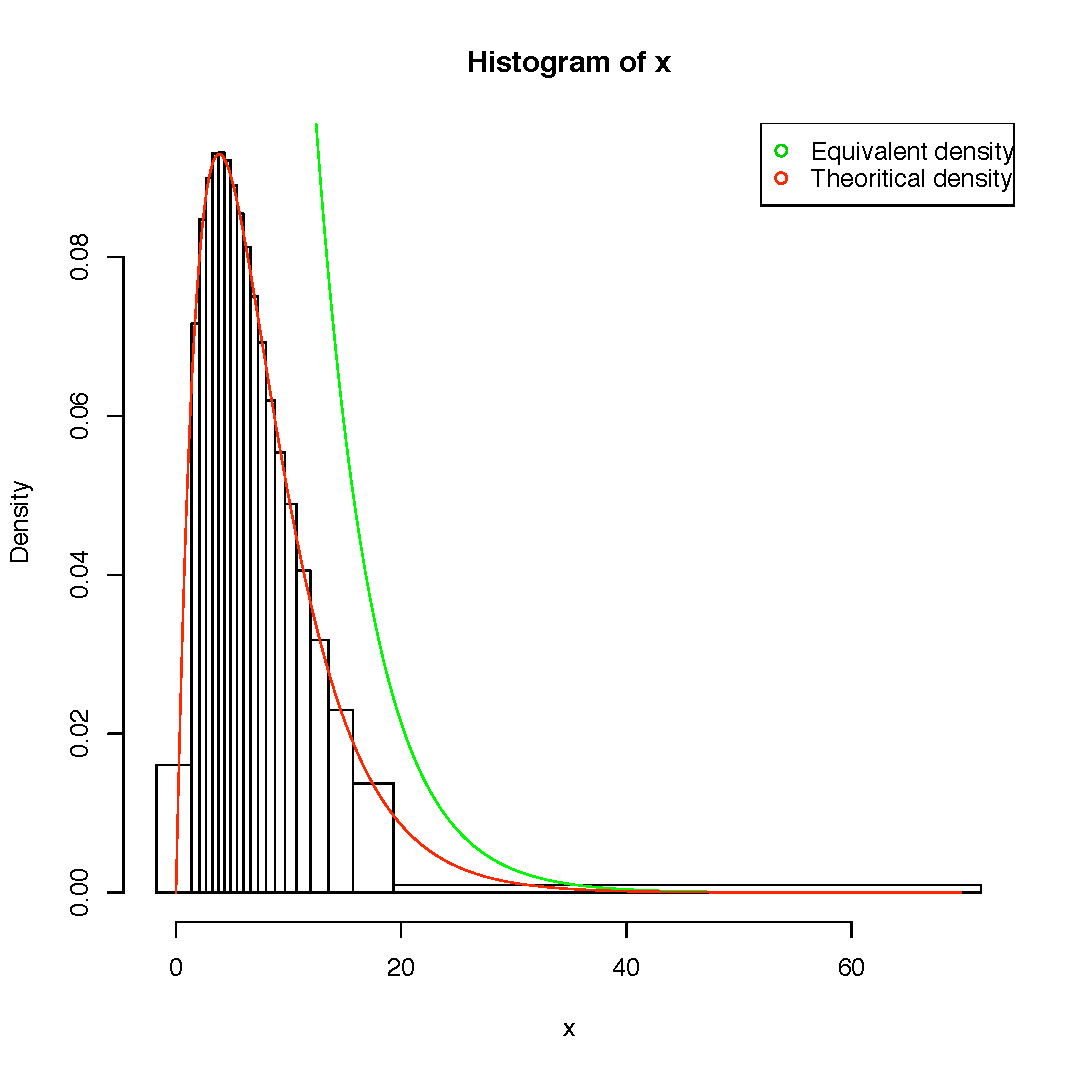
\includegraphics[width=7cm]{image_mod1_exp13_exp15_1000_1000.pdf} 


&

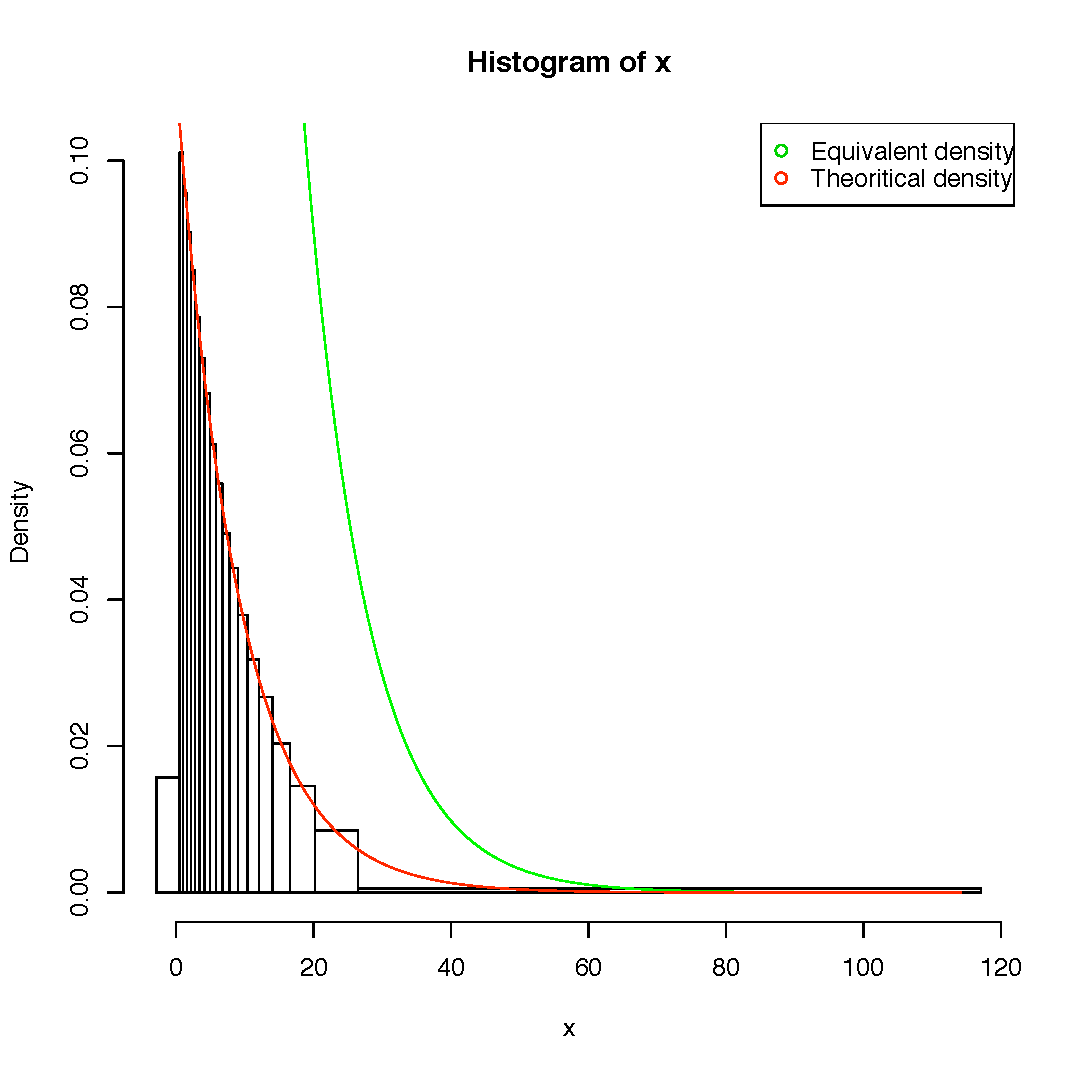
\includegraphics[width=7cm]{image_mod1_exp13_cst13_1000_1000.pdf} 


\end{array}
$
\caption{The sequence of $(X_i)_i$ has an exponential distribution with parameter $\lambda=\frac{1}{3}$ and 
the sequence of $(Z_i)_i$ has a Bernoulli distribution with a side effect probability $p(x)=1-e^{-\frac{1}{3} x}$ (left) and $p=\frac{1}{3}$ (right). The simulation is made for 1000  beds with 1000 patients on each bed within the framework of the model with conditioned side effects. } 
\label{exp}
\label{cst}
\end{figure}
\end{center}




\begin{center}
\begin{figure}[htb!]
$
\begin{array}{cc}

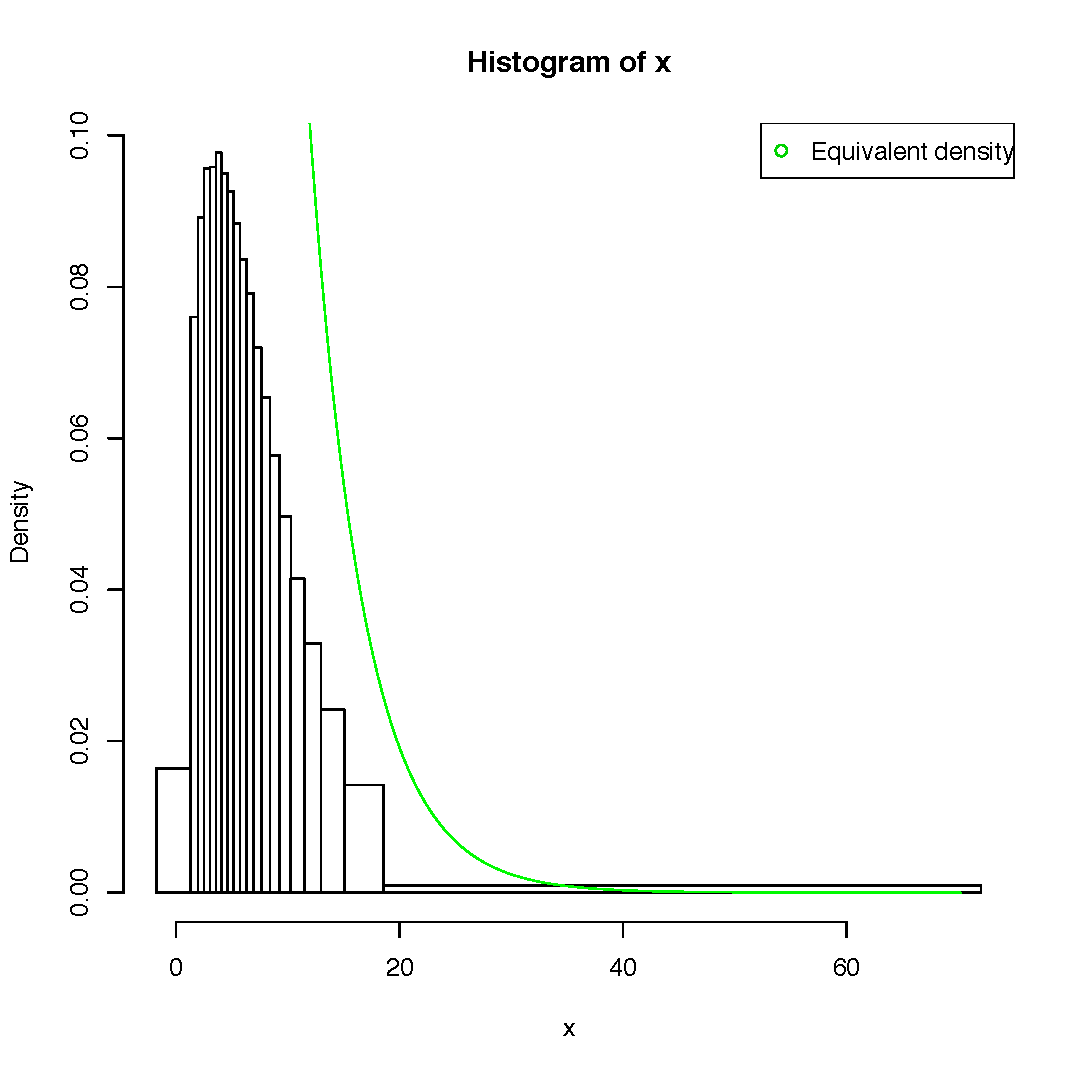
\includegraphics[width=7cm]{image_mod1_exp13_expcomp13_15_110_1000_1000.pdf} 

&

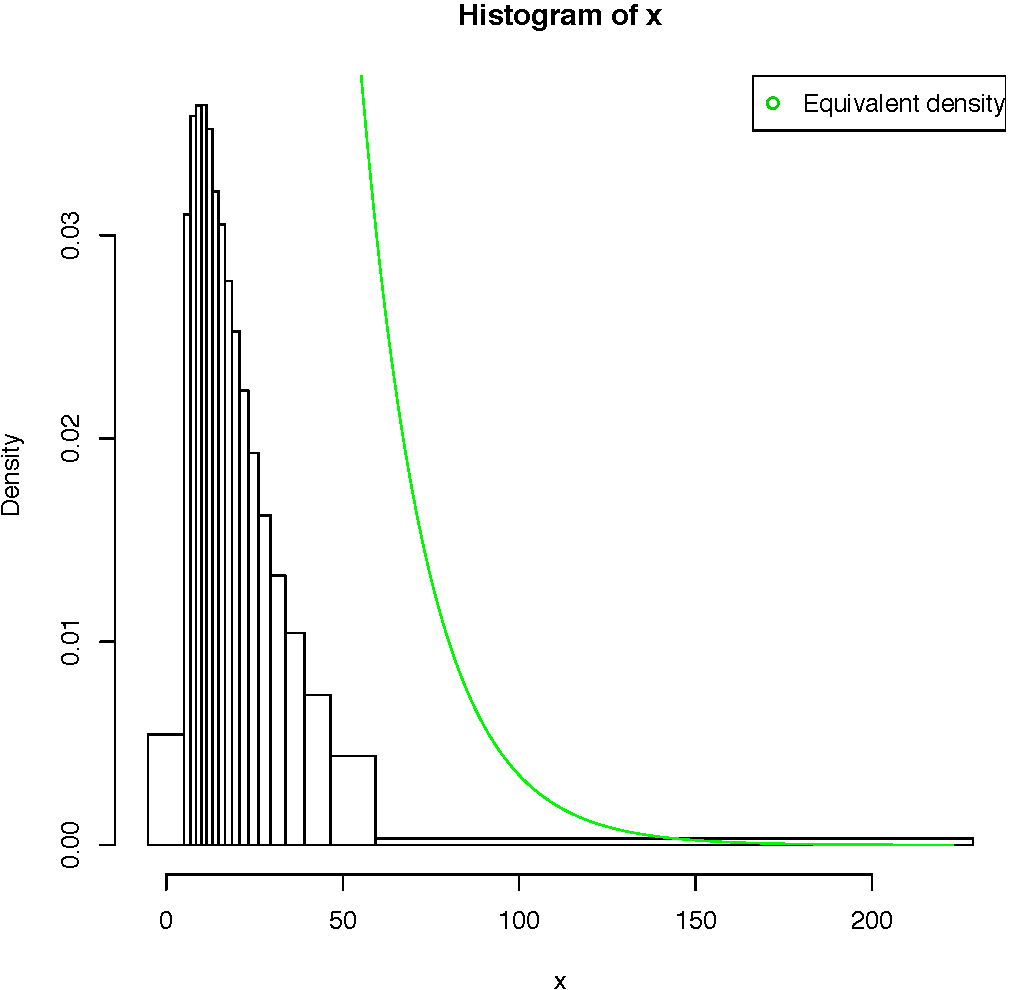
\includegraphics[width=7cm]{image_mod1_exp13_gamma3_13_1000_1000.pdf} 


\end{array}
$
\caption{The sequence of $(X_i)_i$ has an exponential distribution with parameter $\lambda=\frac{1}{3}$ and the sequence of $(Z_i)_i$ has a Bernoulli distribution with a side effect probability $p(x)=1-\frac{1}{3} e^{-\frac{1}{20} x}-\frac{1}{2} e^{-\frac{1}{3} x}-\frac{1}{5} e^{-\frac{1}{10} x}$ (left) and $p(x)$ is a gamma $G(3,1/3)$ distribution function (right). The simulation is made for 1000  beds with 1000 patients on each bed within the framework of the model with conditioned side effects. } 
\label{image_mod1_exp_gamma}
\label{image_mod1_exp_comp}
\end{figure}
\end{center}

We studied the influence of parameters on the equivalent function in three by-models:
\begin{enumerate}
\item{Case where the stay durations $(X_i)_i$ are exponentially distributed and the side effect probability $p$ is constant} 
When the parameters $p$ or $\lambda$ decrease, the equivalent function gets 
closer to the histogramm. That is to say the risk is less overestimated 
when these parameters increases.
\item{Case where the variables $(X_i)_i$ are exponentially distributed and the side effect probability $p(x)=1-exp(-\mu x)$} 
When the parameter $\mu$ or $\lambda$ decrease, the equivalent function moves 
avawy from the histogramm. That is to say the risk is more overestimated 
when these parameters increases.
\item{Case where the variables $(X_i)_i$ are exponentially distributed and the side effect probability $p(x)=1-p_1 e^(-\mu_1 x)-p_2 e^(-\mu_2 x)-p_3 e^(-\mu_3 x)$} 
When the parameter $(\mu_i)_{i\in{1,2,3}}$ or $\lambda$ decrease, the equivalent function moves 
away from the histogramm. That is to say the risk is more overestimated 
when these parameters increase.
\end{enumerate}




\subsubsection{Two examples not exponentially distributed stay durations: lognormally or uniformly distributed }
Let us consider other distributions for the duration variable $X_i$. For example, $Y_i$ may follow 
an uniform distribution, but the uniform distribution does not have the same properties as
the exponential has. Actually, the exponential distribution is the only distribution of
a positive random variable, where the calculi are easy: that is to say that $T=\sum_{i=1}^N X_i$ 
is not a known distribution. Furthermore, equations that have been developped are no longer verified.
However, we make simulations in order to check that $T$ is not too far from an exponential
distribution. We simulate two cases : 
\begin{itemize}
\item{The stay durations $(X_i)_i$ are uniformly distributed }
\item{The stay durations $(X_i)_i$ are lognormally distributed }
\end{itemize}
The figure \ref{image_mod1_nonexp} is a simulation of this model for 1000 beds with
1000 patients on each bed. We can notice on the figure \ref{image_mod1_nonexp} that the
distribution of $T$ is not far from an exponential distribution. In consequence,
the theory developped until here is not far-fetched.

We plot a probability plot of those simulations in order to test the adequacy of $T$
to an exponential distribution with these distributions for the stay durations. We can conclude  from these probability plots that in the case of a lognormal distribution, the variable 
$T$ is nearly an exponential distribution 

\begin{center}
\begin{figure}
$
\begin{array}{cc}
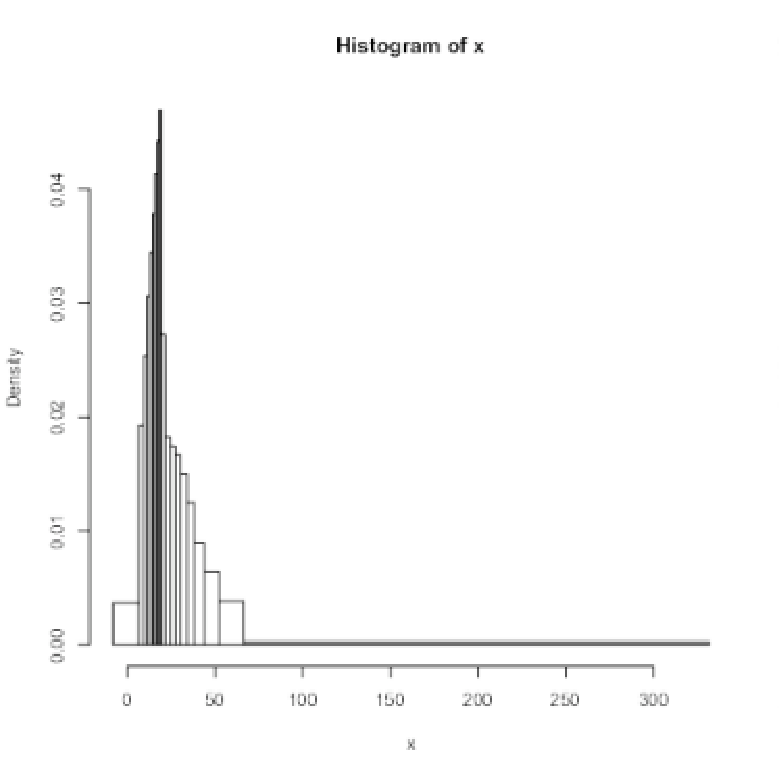
\includegraphics[width=8cm]{image_adequat_exp120_unif020.pdf} & 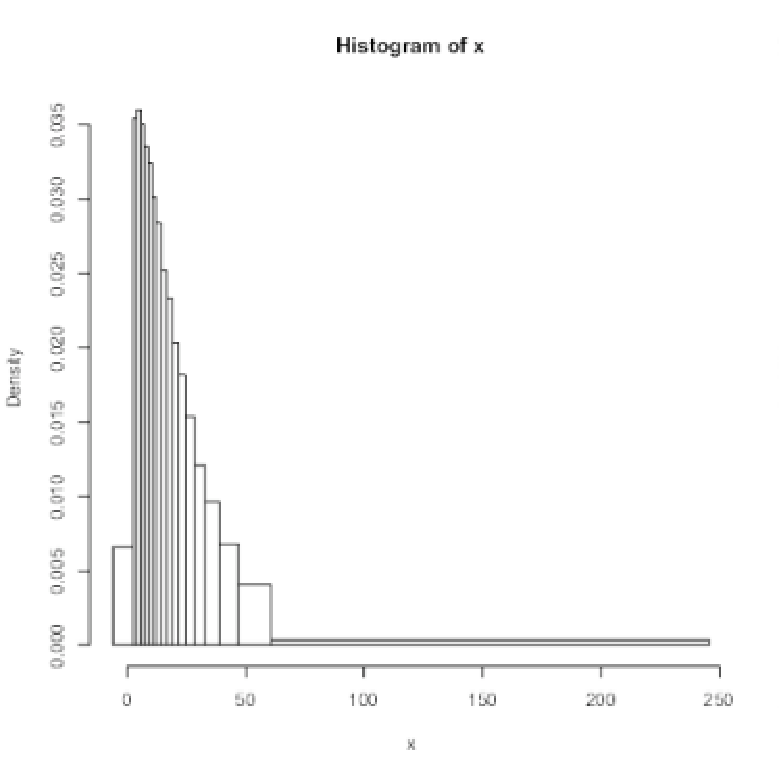
\includegraphics[width=8cm]{image_adequat_exp13_lnorm14_1.pdf} 
\end{array}$
\caption{The distribution of the random variable $T$ when the sequence of $(X_i)$ has an uniform distribution (left) or a lognormal distribution (right) } 

\end{figure}
\label{image_mod1_nonexp}
\end{center}


\subsubsection{Simulation of the model with random side effect}
Unitl here, we study the simulation of the model with conditionned side effect, let us consider the simulation of the model with random side effect.


We simulate this model where the sequence of the random variables $(X_i)_i$
are not censored the variable $Y_i$. We plot the histogram of the random
variable $T$ and the equivalent function (in this case, we can do it).

\begin{figure}[htb!]
\begin{center}
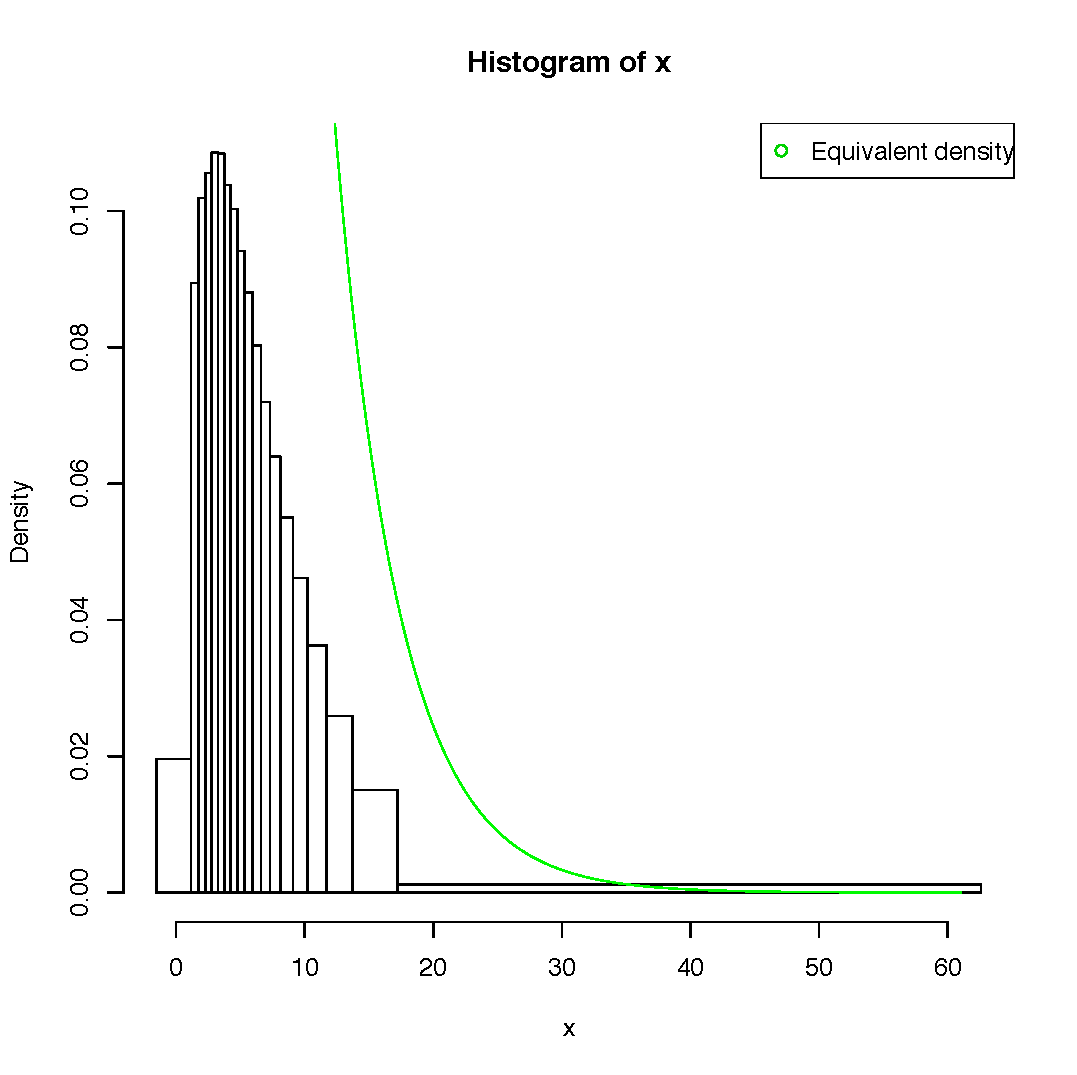
\includegraphics[width=6cm]{image_mod2_exp13_exp15.pdf} 
\end{center}
\caption{ The sequence of $(X_i)_i$ has an exponential distribution with parameter $\lambda=1/3$ and 
the sequence of $(Y_i)_i$ has an exponential distribution with parameter $\mu=1/5$. The simulation is made for 1000  beds with 1000 patients on each bed within the framework of the model with random side effects.} 
\label{image_mod2}
\end{figure}


\subsection{The De Vielder's approximation}

In 1978, De Vielder proposed an approximation based on the idea to replace an unknown risk process with 
a process with exponentially distributed claims. His idea was to identify the three first moments. \\

In our study, the "De Vielder's model" is the one where the sequence of $(X_i)_i$ has an exponential 
distribution with parameter $\lambda$ and the sequence of $(Z_i)_i$ has a Bernoulli distribution 
with a side effect probability $p(x)=1-e^{-\mu x}$.\\

Indeed, in that case, we are able to express the distribution function, the moments and the risk constants. We know : 
$$A(t) =  \frac{1}{\lambda - \mu}(\lambda e^{-\mu t}-\mu e^{-\lambda t})$$
\begin{equation}
E[T]= m_1 = \frac{\lambda+\mu}{\lambda \mu} ~ \textrm{ and } ~ E[T^2]= m_2 = \frac{1}{\lambda^2}+\frac{1}{\lambda \mu}+ \frac{1}{\mu^2} 
\label{DV_moments}
\end{equation}

\begin{equation}
R=\mu ~ \textrm{ and } ~ C_R=\frac{\lambda}{\mu}(1-\frac{\lambda}{\mu-\lambda})
\label{eq_DV}
\end{equation}

In our work, in order to apply the De Vielder's approximation, we identify the two first moments $m_1$ 
and $m_2$ of the "De Vielder's model" with the two first moments $\xi_1$ and $\xi_2$ of the
random variable $T$, calculated from the data.\\ 

As a result, we look for $\mu$ and $\lambda$ such as :
$\left\{ 
\begin{array}{c}
\xi_1=m_1\\
\xi_2=m_2
\end{array}
\right.
\Leftrightarrow 
\left\{
\begin{array}{c}
\xi_1=\frac{\lambda+\mu}{\lambda \mu}\\
\xi_2=\frac{1}{\lambda^2}+\frac{1}{\lambda \mu}+ \frac{1}{\mu^2} 
\end{array}
\right.$\\

We are able to solve this system of two equations with two unknowns. As shown in appendix \ref{DV}
page \pageref{DV}, the discriminant of the second-order equation could be negative. 
Furthermore, in the case of a positive discriminant, we choose the smallest positive root for $\mu$.
Then the value of $\lambda$  is known. Let us denote by $\stackrel{\sim}{\lambda}$ and $\stackrel{\sim}{\mu}$
the "De Vielder" values of $\lambda$ and $\mu$.\\

We compute $\stackrel{\sim}{\lambda}$ and $\stackrel{\sim}{\mu}$ in several cases and it appears
that the discriminant is negative when $p(x)$ is a gamma, lognormal and a uniform distribution function. 
However, in other cases, $\stackrel{\sim}{\lambda}$ and $\stackrel{\sim}{\mu}$ can be calculated.



\subsection{An inference of the risk constant $R$}
In this paragraph, we study two methods to estimate the risk constant R : 
\begin{itemize}
\item{The first approach is a parametric estimate of R, when we suppose the sequence of $(X_i)_i$ is exponentially distributed and the side effect probability $p(x)$ is $1-e^{-\mu x}$  }
\item{In the second method, we don't make any hypothesis on the side effect probability, but we solve the equation $(\star)$ with the help of the Bayes formula} 
\end{itemize}
\subsubsection{A parametric method}
We assume that the sequence of $(X_i)_i$ is exponentially distributed with parameter $\lambda$.The 
parameter inference consists in solving the equation $(\star)$ , 
assuming that $q(x)=exp(-\mu x)$. In consequence, we can express the distribution of $T$ :  
$F_T(t)=1-\frac{1}{\lambda - \mu}(\lambda e^{-\mu t}-\mu e^{-\lambda t})$ that is to 
say $A(t)=\frac{1}{\lambda - \mu}(\lambda e^{-\mu t}-\mu e^{-\lambda t})$. 
The likelihood function $L$ for the sequence $(Z_i / X_i=x_i)_i$ is worth :
$$
L(\mu,x_1,\dots,x_n,z_1,\dots,z_n) = \prod_{i=1}^n (e^{-\mu x_i})^{1-z_i}(1-e^{-\mu x_i})^{z_i}
$$
$$
ln(L)(\mu,x_1,\dots,x_n,z_1,\dots,z_n) = \sum_{i=1}^n (-\mu x_i)(1-z_i)+  \sum_{i=1}^n(z_i)ln(1-e^{-\mu x_i}) 
$$
Thanks to the log-likelihood, we are able to compute the estimator of the maximum of likelihood of $\mu$. 
Hence, the parametric estimator of $R$ is the estimator of the maximum of likelihood of $\mu$ 
(see the De Vielder approximation). Furthermore, we can also compute the survival function from the data 
in addition to the asymptotic function.
 


\subsubsection{A non parametric method}

We assume that the sequence of $(X_i)_i$ is exponentially distributed of parameter $\lambda$.The non 
parametric inference consists in solving the equation $(\star)$ without making any hypothesis on the probability $q(x)$. 
We recall that $(\star)$ $ \Leftrightarrow \lambda Lq(\lambda-R) = 1$ where
$Lq(r) = \int_0^{\infty} e^{-r x }q(x) dx$.
We obtain :
$$
P(Z=0)E(e^{-r X}/Z=0) = 1
$$
Replacing $P(Z=0)$ by  $\frac{1}{n}\sum_{i=1}^n {1\!\!1}_{\{0\}}(z_i)$, 
and $E(e^{-r X}/Z=0)$ by $\frac{1}{n}\sum_{i=1}^n e^{r x_i}{1\!\!1}_{\{0\}}(z_i)$ 
leads to the equation (appendix \ref{mod1_non_param} page \pageref{mod1_non_param}):

$$ \frac{1}{n}\sum_{i=1}^n {1\!\!1}_{\{0\}}(z_i) \frac{1}{n}\sum_{i=1}^n e^{r x_i}{1\!\!1}_{\{0\}}(z_i) =1 $$ 

Solving this equation numerically thanks to the \texttt{R} function 
\texttt{optimize} we find an estimate of
the risk constant $R$. Unlike the previous method, we do not make any hypothesis on the
side effect probability $p$. In consequence, we expect better results when $q(x)$ is not an 
exponential distribution function (general case) with this method than the previous one.
But this is the opposite when $q(x)$ is not far from an exponential distribution function.


We numerically estimate the bias, the variance, $R$ and $C_R$ for the non parametric estimator, 
the parametric estimator and the De Vielder estimator in six different side effect probability cases :
\begin{enumerate}
\item{$p(x)$ is a exponential distribution function}
\item{$p(x)$ is a constant function}
\item{$p(x)$ is a mix of exponential distribution function} 
\item{$p(x)$ is a gamma distribution function}
\item{$p(x)$ is a lognormal distribution function}
\item{$p(x)$ is a uniform distribution function}
\item{$p(x)$ is a weibull distribution function}
\end{enumerate}
To make this simulation comparable, we simulate the model with conditioned side effects with $(X_i)_i \sim \varepsilon(1/3)$ and the side effect probability $p(x)$ has a mean of $20$ for each case or the closest mean to $20$. Furthermore, we estimate the risk constant on 100 samples in each case
with 1000 patients for each sample.
\begin{verbatim}
1.
           nonpar           par
bias 4.407856e-02 -3.503516e-06
var  6.001352e-05  1.972828e-05
R    9.405885e-02  4.997679e-02
CR   8.492920e+00  1.455619e+01

2.
           nonpar          par
bias 1.575410e-02 4.573187e-04
var  1.714712e-05 5.675577e-06
R    3.242554e-02 1.712875e-02
CR   2.197198e+01 4.066553e+01

3.
           nonpar           par
bias 3.247060e-02 -5.558817e-05
var  4.621880e-05  1.006148e-05
R    6.880894e-02  3.628275e-02
CR   1.101930e+01  1.967524e+01

4.
           nonpar           par
bias 1.832645e-02 -7.552530e-04
var  2.267637e-05  7.363311e-06
R    3.778277e-02  1.870107e-02
CR   1.911443e+01  3.773611e+01

5.
           nonpar          par
bias 4.556463e-02 1.017082e-03
var  7.013414e-05 3.104221e-05
R    1.005464e-01 5.599889e-02
CR   8.101552e+00 1.318976e+01

6.
           nonpar          par
bias 2.514426e-02 2.598740e-04
var  3.878331e-05 1.073282e-05
R    5.236710e-02 2.748271e-02
CR   1.408411e+01 2.580822e+01

7.
           nonpar          par
bias 4.588473e-03 1.540856e-04
var  5.405285e-06 1.589171e-06
R    9.367470e-03 4.933083e-03
CR   7.709814e+01 1.468196e+02
\end{verbatim}
 
The most suprising result is that the parametric estimation has the smallest
bias in each cases. From this simulation, we can conclude that the parametric 
estimation is better than the non parametric one in terms of bias and variance with those parameters. Other tests with other distributions or parameter values would be very wise to conclude that the parametric estimation is better than the non-parametric one.

\subsection{A variant of the Kaplan-Meïer estimate}

In this subsection, we explain how we adapt the Kaplan-Meïer method in order to plot the survival function $A(t)$.\\

We propose a variant of Kaplan-Meïer estimate that offers a way of building the curve of the survival function from data about duration stays in hospitals. 
One principle lies at the very heart of this approximation : the survival function remains constant between two successive distincts moments with side effects.\\

A plot of the approximated survival function $\hat A $ is a serie of horizontal steps of declining magnitude which, when a large enough sample of patients is taken, approaches the true survival function for that population. An important advantage of the Kaplan-Meïer curve is that the method can take into account censored data. Indeed, only the patients without full-blown side effects are still being observed.\\

Let us consider for $i$ in  $\left\{ 0,..,n \right\}$, assuming that $i$ stands for the $i^{th}$ time observed:
\begin{itemize}
 	\item $D$ vector such as $D(i)$ is the number of patients with side effets arisen before the time $i$
   \item $N$ vector such as $N(i)$ is the number of patients that have not had 
side effets arisen before the time $i$
   \item $\hat A$ vector such as $\hat A(i)$ is the survival function at the time $i$
   %\item TH vector such as TH(i) is the theoretical simulation at the time i 
%of the theoretical survival function
\end{itemize}

Then, in order to plot the survival function, we work out the instantaneous risk $h(t)$. It is worth :
\begin{equation}
h(t)=lim_{dt\rightarrow 0}\frac{P(T<t+dt)/ T \geq t}{dt}
\end{equation}
As a result, we have $\hat h(i)=\frac{D(i)}{N(i)}$
%le numérateur exprime la probabilité pour qu'un individu décède juste après le temps t sachant qu'il était vivant à cet instant. Le risque instantané est donc une probabilité conditionnelle par unité de temps ; il exprime à chaque instant la « force de mortalité ».

%Connaître la variable aléatoire T, c'est connaître sa fonction de survie, puisqu'elle n'est autre que 1 - sa fonction de répartition.

Let us build the survival function assuming that the survival function between successive distinct sampled observations is constant.
\begin{enumerate}
	\item When $t=0$, $\hat A(0)=1$
	\item For $i$ in $\left\{ 0,..,n \right\}$, between $t=i$ and $t=i+1$, 	
		\begin{itemize}
			\item If no side effect has arisen, $\hat A(i+1)=\hat A(i)$
			\item If a side effect has arisen, $\hat A(i+1)=(1- \hat h(i+1))A(i)$ with $\hat h(i+1)=\frac{D(i+1)}{N(i+1)}$\\
			that is to say that : $$
			\hat A(i) = \prod_{j=0}^{i}(1-\hat h(i))
			$$
		\end{itemize}
\end{enumerate}

It is difficult to get a feel for the reliability of the curve, especially towards the end. However, we can notice a quite good approximation at the beginning of the approximation. That is interesting because we are especially interested in the value of the survival function at small times. Indeed, we can suppose that most of the patients stay in hospital less than about ten days.

% graphes à reprendre

\begin{center}
\begin{figure}
$\begin{array}{cc}
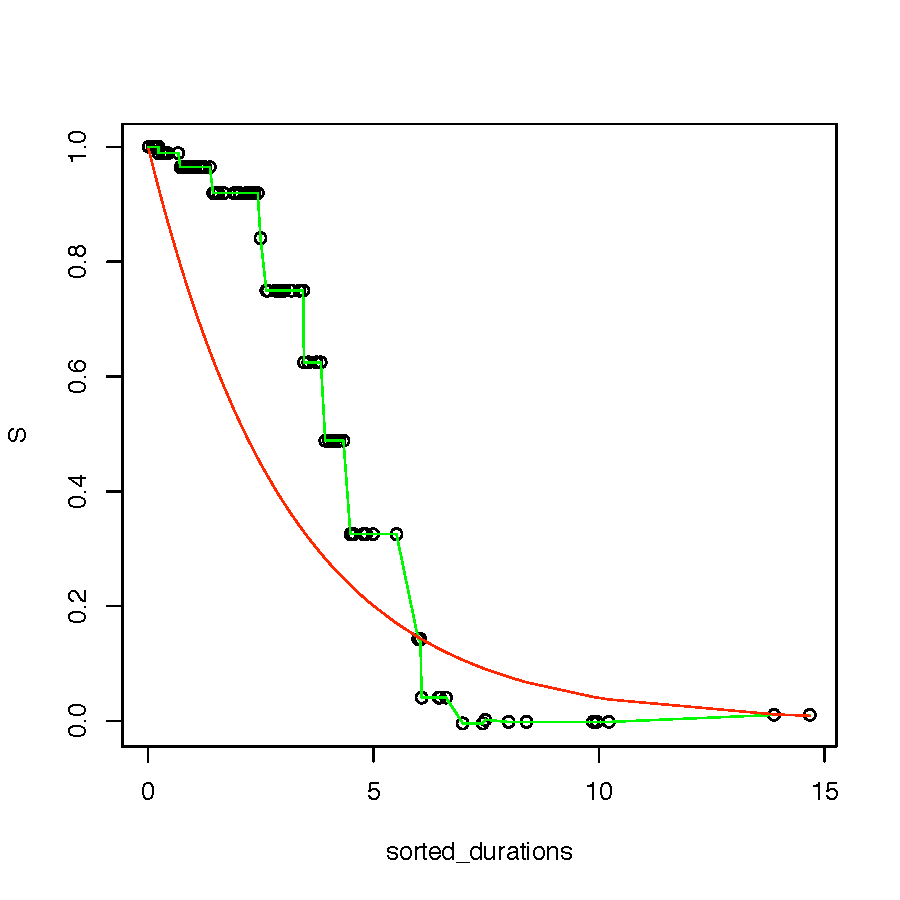
\includegraphics[width=8cm]{d100exp_exp.pdf} & 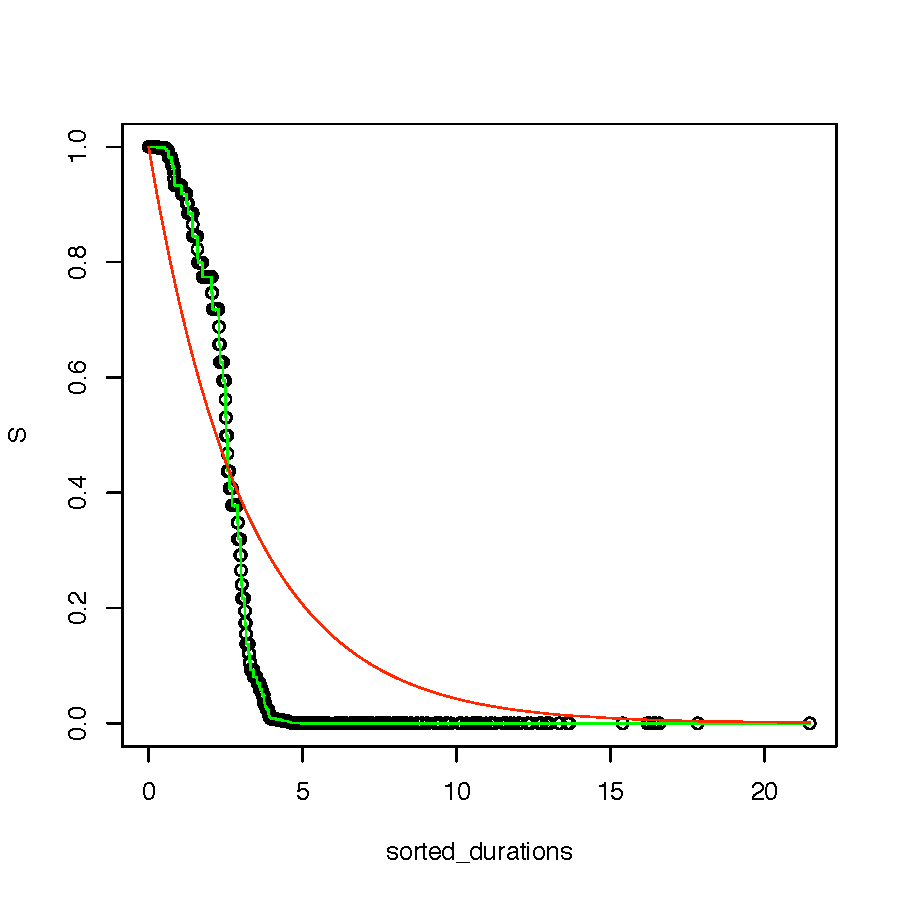
\includegraphics[width=8cm]{d1000exp_exp.pdf} \\
\end{array}$
\caption{The Kaplan-Meier's variant estimation with $100$ and $1000$ patients, and $(X_i) \sim \varepsilon(\lambda)$ and $p \sim \varepsilon(\mu)$. The green plot is the survival function got thanks to our study ; the red one is the theoretical one.} 
\end{figure}
\label{estim_KM_eps}
\end{center} 

\clearpage
\section{The \texttt{rhosp} package}
\label{package}
In this section, we will describe the implementation of the \texttt{R} functions in
order to simulate our problem and estimate the risk constant of our models.

We made an \texttt{R} package to let our functions available through Comprehensive R Archive Network. Here is a brief description of 
our main functions. Actually, we have two files \texttt{simul.R} and \texttt{estim.R}.


\subsection{A simulation file : \texttt{simul.R}}
The main goal of the file \texttt{simul.R} is obviously to simulate our 2 models
: \textsl{model with conditioned side effects} and \textsl{model with random side effects}.
In order to guarantee a multi-purpose functions, we do our best to have the 
most general arguments for our functions. That is why the following functions have 
a list in argument to describe the distribution of the variable $X_i$ and 
the pseudo-distribution of the side effect probability $p$.

\begin{itemize}

	\item{\begin{footnotesize}\begin{verbatim}	histo<-function(X,disXi=NULL,disP=NULL,plotDV=FALSE)	\end{verbatim}\end{footnotesize}}
	The function \texttt{histo} plots the histogram of the object $X$ whose components are the variable $T$, the estimates $R$, $C_R$, $\lambda$ and $\mu$ estimated with De Vielder approximation. The argument disXi is a three-elements list : rangen (a random positive variable generator),
	       nbparam (number of parameter of this distribution) and param (a list of its parameters). disP is also a three-element list to describe the side effect probability.
	\item{\begin{footnotesize}\begin{verbatim}	mainSimul<-function(nbBed,nbPatient,disXi,disP,toplot=FALSE,calc=TRUE)	\end{verbatim}\end{footnotesize}}
	The function \texttt{mainSimul} simulates \texttt{nbBed} times the \textsl{model with conditioned side effects} with our function \texttt{simul}
	and calculates the risk constant $R$ and $C_R$ by solving the renewal equation $(\star)$. This renewal equation is only valid if the $X_i$ forms a poisson process.
	
	\item{\begin{footnotesize}\begin{verbatim}	makeSample<-function(file, nbPatient,disXi,disP)	\end{verbatim}\end{footnotesize}}
	The function \texttt{makeSample} write a simulation in a given file. This file can be used by the estimation functions.
	
	\item{\begin{footnotesize}\begin{verbatim}	mainSimul2 and makeSample2	\end{verbatim}\end{footnotesize}}
	These two functions concerning the model with random side effects plays the same role as 
	\texttt{mainSimul} and \texttt{makeSample} did in the model with conditioned side effects.
	
\end{itemize}


\subsection{An estimation file : \texttt{estim.R}}
The main purpose of the file \texttt{estim.R} is to compute the estimators
described in the previous section and quantify their quality. Each estimation function
takes in an argument a file of data, and have some optional arguments. We suppose that
the data are sorted in three columns, one for the cumulated number of the patient, one 
for the stay duration  of a patient and another for a side effect report.

\begin{itemize}
	\item{\begin{footnotesize}\begin{verbatim}	DV<-function(T)	\end{verbatim}\end{footnotesize}}
	The function \texttt{DV} computes the De Vielder's approximation on a vector \texttt{T}, 
	which is the vector of the observations of the variable $T$. This auxiliary function is used in the following functions.
	\item{\begin{footnotesize}\begin{verbatim}	estimParam<-function(file,toplot=TRUE,header=TRUE)	\end{verbatim}\end{footnotesize}}
	The function \texttt{estimParam} computes the parametric estimation over the data given in the file \texttt{filename}.
	There are also the functions \texttt{estimNonParam} and \texttt{estimDV} which compute 
	the non parametric estimation and the De Vielder estimation respectively.
	\item{\begin{footnotesize}\begin{verbatim}	calcBiasParam<-function(file,nb=10,disXi=arg1Exp,disP=arg2Exp)	\end{verbatim}\end{footnotesize}}
	The function \texttt{calcErrorParam} calculate the bias and the variance of the parametric estimator.
	There are also the functions \texttt{calcErrorNonParam} and \texttt{calcErrorDV} which compute the same things with
	the non parametric estimator and the De Vielder estimator respectively.
	\item{\begin{footnotesize}\begin{verbatim}	Table<-function(file,nb=10,mod)	\end{verbatim}\end{footnotesize}}
	The function \texttt{Table} makes arrays of bias, variance, $R$ and $C_R$ for the different estimators
	in different cases in order to compare these estimators.
\end{itemize}

\clearpage

\section{Conclusion}
\label{conclusion}
First, we studied two models : the model with conditioned side effects and the model with random side effects. We focused on the duration of a patient stay in hospital.  We look at one hospital bed and we observe 
the successive times of stay in order to get the risk constant $R$. Since we did not always manage to obtain an explicit expression of $R$, we took an interest in estimating the risk constant and in quantifying and valuing his quality. We made this thanks an \texttt{R} package we create. We can notice that we found a good method -- the parametric one -- to approximate $R$.\\

Of course, it is easy to make the models more complex. Most of the time, we will not be able to study them if they have new amendments. However, some more complex models are easy to study. For instance, the risk constant $R$ can vary according to seasons. For example, we can sense 
that patients stays are longer during the winter. Thus, we should solve an unclassical issue, i.e. with a sequence of stay durations $(X_i)_i$ exponentially distributed with parameter $\lambda(t)$. The renewal process described by the sequence of stay durations is a non homogeneous Poisson process. However, we can find again the classical model by applying a change in variables. Then, the model reacts as if the time were accelerated. Actually, this time dilatation can stand for periodic variations in the risk factor. \\

Finally, we could think that we could apply in reality our study. Indeed, given that even if the stay durations are not exponentially distributed, $T$ is not far from an exponential tail, we could use our work to find the risk constant during hospitalization. One thing to do would be to apply our work on real hospital data in order to verify its accuracy. This could help health services to control hospital costs  and physicians to prenvent patients from hospital side effects such as nosocomial infections and venous thrombosis. 

\clearpage

%references
\section{References}
\begin{itemize}
	\item \textsl{Aspect of risk theory}, Jean Grandell, 1991
	\item \textsl{Cours de processus aléatoire de deuxième année \textsc{Ensimag}}, Olivier Fran\c cois, 2004
	\item \textsl{http://tolstoy.newcastle.edu.au/R/help/04/03/index.html}
	\item \textsl{http://en.wikipedia.org/wiki/Kaplan-Meier\_estimator}
\end{itemize}



\newpage
 \section{Appendix}
% \printindex



\footnotesize{
\appendix

%%%%%%% appendix


\section{Distribution of T in the first model with $X_i \sim \epsilon(\lambda)$
 and $Z_i \sim B(p)$ with a constant side effect probability $p$ }

\label{mod1_dem1}

It is easy to see $N$ is a geometric distribution.
\begin{equation}
LT(z)=E(e^{-zT})=E(E(e^{-z\sum_{i=1}^N X_i}/N))
\end{equation}
\label{eq}
Moreover $E(e^{-z\sum_{i=1}^N X_i}/N=n) = E(e^{-z\sum_{i=1}^N X_i})$ is
the Laplace tranform of a gamma distribution of parameter $n$ and $\lambda$.
Since the Laplace tranform of a sum of random variables is the product of
the Laplace tranforms of the random variables, we have $E(e^{-z\sum_{i=1}^N X_i}/N=n) 
= \frac{\lambda}{\lambda+z}^n$. It follows then from \ref{eq} that
$LT(z) = E(\frac{\lambda}{\lambda+z}^N) = G_N(\frac{\lambda}{\lambda+z})$ where
$G_N$ is the generator function of  $N$ ($G_N(z)=\frac{pz}{1-(1-p)z}$).
Hence, 
$$
LT(z) = \frac{\lambda p}{\lambda p + z}
$$
This proves that $T$ is an exponential distribution of parameter $\lambda p$.


%%%%%%%%%% appendix
\section{Distribution of T with an expression of the survival function}
\label{mod1_dem2}

$$P(T>t/X_1=x) = P(T>t/X_1=x,T>X_1)P(T>X_1) + P(T>t/X_1=x,T=X_1)P(T=X_1)$$
			$$= P(T>t/X_1=x,T>X_1)q(x) + P(T>t/X_1=x,T=X_1) (1 -q(x))$$
			$$= P(T>t-x+x/T>x)q(x) + 1\!\!1_{\{x>t\}}(1-q(x))$$
Because of the lack of memory of the exponential distribution of$(X_i)_i$,
we have $P(T>t/X_1=x) = P(T>t-x)q(x) + 1\!\!1_{\{x>t\}}(1-q(x))$
$$A(t) = \int_{\mathbb{R}} P(T>t/X_1=x) f_{X_1}(x) dx = \int_0^{\infty} [P(T>t-x)q(x) + 1\!\!1_{\{x>t\}}(1-q(x))] \lambda e^{-\lambda x} dx$$
$$A(t) = \int_0^t A(t-x)q(x)\lambda e^{-\lambda x} dx + \int_t^{\infty}[A(t-x)q(x)+1-q(x)] \lambda e^{-\lambda x} dx$$
$$A(t) = \int_0^t A(t-x)q(x)\lambda e^{-\lambda x} dx + \int_t^{\infty}[1] \lambda e^{-\lambda x} dx 
= 1-F(t)  + \int_0^t A(t-x)q(x)\lambda e^{-\lambda x} dx$$

Let $h(x) = q(x)\lambda e^{-\lambda x}$.
We can apply the Laplace transform to the previous equation:
$$LA(s) = \frac{1}{s} - (\frac{1}{s}-\frac{1}{\lambda+s}) + LA(s).Lh(s)$$ 
Thus we have 
$LA(s) = \frac{1}{\lambda+s}. \frac{1}{ 1-Lh(s)}$.


When $q(x) = e^{-\mu x}$, we can verify that $A(t) = \frac{1}{\lambda-\mu}(\lambda e^{-\mu t}-\mu e^{-\lambda t})$
because the function $t\rightarrow\frac{1}{\lambda-\mu}(\lambda e^{-\mu t}-\mu e^{-\lambda t})$ has the same Laplace transform
as $A$ and the Laplace transform is injective.

%%%%%%% appendix
\section{The renewal equation for the survival function }
\label{mod1_dem3}

Let $B(t) = e^{Rt} A(t)$ where $R$ is the positive solution of the equation $\lambda Lq(\lambda-r) =1$ , for $r$ in $(0,\lambda)$.
Thus, $B(t) = e^{Rt}(1-F(t))  + \int_0^t B(t-x)q(x)\lambda e^{-(\lambda-R) x} dx$. Since R verifies the previous,
the function $t\rightarrow g(t)=q(t)\lambda e^{-(\lambda-R) t} $ is a density. Hence, $B$ is solution of the following renewal equation:
$$
B(t) =  e^{Rt}(1-F(t))  + \int_0^t B(t-x)dG \textrm{  where  }G'(t)=g(t)
$$
Thanks to the renewal theorem, we obtain a limit of $B$ when $t\rightarrow + \infty$:
$B(t)= \frac{1}{\mu} \int_0^{\infty} e^{Rt}(1-F(t))dt$ 
where $\mu=\int_0^{\infty}x g(x)dx = \lambda L(x\rightarrow x q(x))(\lambda-R) = \lambda (-1)L'q(\lambda-R) = -\lambda \frac{-1}{\lambda^2}=\frac{1}{\lambda}$.
Hence, $B(t)=\lambda (\frac{1}{R}(1-\frac{\lambda}{R-\lambda}))$. Finally, we obtain an asymptotic of the function $A$:
$$
A(t)= \frac{\lambda}{R}(1-\frac{\lambda}{R-\lambda}) e^{-Rt}
$$



%%%%%%% appendix 1
\section{Probability of success for $Z_i \sim \varepsilon(\mu)$ }
\label{mod2_dem1}


The integration of the density function of the couple ($X_i$,$Y_i$) over $D= \{(x,y)\in \mathbb{R_+}^2,y\leq x\}$ yields
$$
P(X_i>Y_i)=\int P(X_i>y)f_{Y_i}(y) dy = \int P(X_i>y) \mu e^{-\mu y} dy=\int  \mu e^{-(\lambda+\mu) y} dy=\frac{\mu}{\lambda+\mu}
$$


%%%%%%% appendix 2
\section{Probability of success for any $Z_i$}
\label{mod2_dem2}

The  integration of the density function of the couple ($X_i$,$Y_i$) over $D= \{(x,y)\in \mathbb{R_+}^2,y\leq x\}$ yields
$$
P(X_i>Y_i)=\int \int_D f_{X_i,Y_i}(x,y) dx dy = \int \int_D f_{X_i}(x) f_{Y_i}(y) dx dy = \int_0^{\infty} \int_0^x f_{X_i}(x) f_{Y_i}dy dx
$$
Thus we have
$$
P(X_i>Y_i) = \int_0^{\infty} f_{X_i}(x) F_{Y_i}(x) dx = E(F_{Y_i}(X_i))
$$

%%%% appendix
\section{Solving the De Vielder system}
\label{DV}
We recall the "De Vielder" system:
$$
\left\{
\begin{array}{c}
\xi_1=\frac{\lambda+\mu}{\lambda \mu}\\
\xi_2=\frac{1}{\lambda^2}+\frac{1}{\lambda \mu}+ \frac{1}{\mu^2}
\end{array}
\right.
\leftrightarrow
\left\{
\begin{array}{c}
\xi_1=\frac{\lambda+\mu}{\lambda \mu}\\
\xi_2=\frac{2\mu^2+2\mu\lambda+2\lambda^2}{\lambda^2\mu^2}
\end{array}
\right.
\leftrightarrow
\left\{
\begin{array}{c}
\lambda=\frac{\mu}{\mu\xi_1-1}\\
\xi_2 \mu^2 (\frac{\mu}{\mu\xi_1-1})^2 = 2\mu^2+2(\frac{\mu}{\mu\xi_1-1})\mu+2(\frac{\mu}{\mu\xi_1-1})^2
\end{array}
\right.
$$
$$
\leftrightarrow
\left\{
\begin{array}{c}
\lambda=\frac{\mu}{\mu\xi_1-1}\\
\xi_2 \mu^2 (\frac{\mu}{\mu\xi_1-1})^2 = 2\mu^2+2(\frac{\mu}{\mu\xi_1-1})\mu+2(\frac{\mu}{\mu\xi_1-1})^2
\end{array}
\right.
\leftrightarrow
\left\{
\begin{array}{c}
\lambda=\frac{\mu}{\mu\xi_1-1}\\
\frac{\xi_2\mu^2}{2} = (\mu\xi_1-1)^2 + \mu\xi_1-1+1
\end{array}
\right.
$$
Thus we have a second-order equation of the unknown $\mu$ :
$
\mu^2(\frac{\xi_2}{2}-\xi_1^2)+\mu\xi_1-1=0
$
Hence, we obtain $\delta = 2\xi_2-3\xi_1^2$.
$$
\mu=\frac{-\xi_1 \pm \sqrt{2\xi_2-3\xi_1^2}}{2(\frac{\xi_2}{2}-\xi_1^2)}=f(\xi_1,\xi_2)~ \textrm{when} ~\delta>0~ and ~
\lambda=\frac{f(\xi_1,\xi_2)}{f(\xi_1,\xi_2)\xi_1-1}
$$ 




%%%% appendix
\section{A new expression of $(\star)$ }
\label{mod1_non_param}

We apply the Bayes formula to $P(Z=0/X=x)$, thus we have
$$
Lq(r) = \int_0^{\infty} exp(-r x )P(Z=0/X=x)dx = \int_0^{\infty} exp(-r x )\frac{f_X^{Z=0}(x) P(Z=0)}{f_X(x)} dx
$$
$$
Lq(r)		= \frac{P(Z=0)}{\lambda}\int_0^{\infty} exp(-(r-\lambda) x )f_X^{Z=0}(x) dx= \frac{P(Z=0)}{\lambda}E(exp(-(r-\lambda) X)/Z=0)
$$
Hence,
$$
\lambda Lq(\lambda - r) = 1 \Leftrightarrow P(Z=0)E(exp(-r X)/Z=0) = 1
$$


} %fin du footnotesize pour


\end{document}
